%!TEX root = SysSpec_ClockPendulumAnalyzer.tex
\section{Systemdesign}
    Im Kapitel Systemdesign wird die Umsetzung einzelner Komponenten sowie der gesamte Kontext des CPA erklärt.
        \subsection{Kontextdiagramm}
        Der CPA Kontext wird mittels untenstehendem Diagramm dargestellt. Das Projekt umfasst ein tinyK20 als Hardware Counter, ein Raspberry Pi als Recheneinheit und ein Sensor Board auf dem ein Infrarotsensor montiert ist.\\
        Für die Benutzerinteraktion wird ein UserInterface definiert und ein Web Client erstellt. Das UserInterface ermöglicht es weitere Benutzerschnittstellen an den CPA zu hängen. Zum Beispiel eine Qt Applikation.
        \begin{figure}[H]
            \centering
            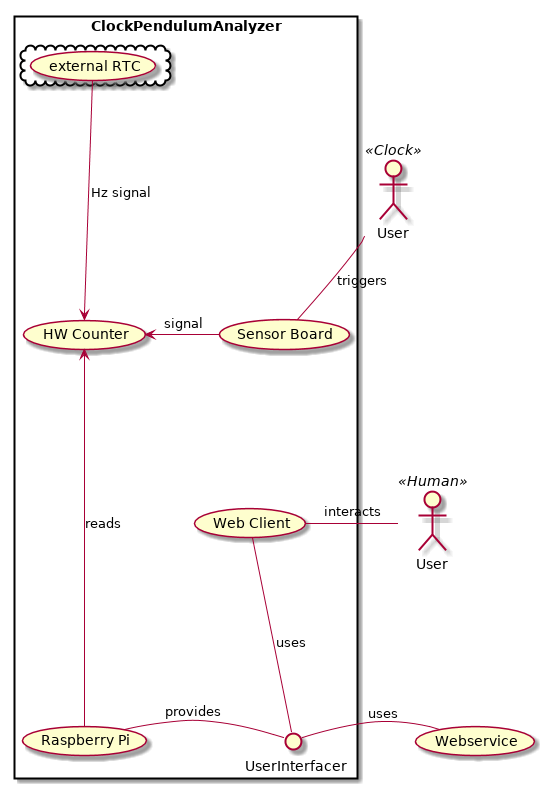
\includegraphics[width=.7\textwidth]{context.png}
            \caption{erweitertes Kontextdiagramm}
        \end{figure}

    	\subsection{Umsetzung des Clock Update}
		\subsection{Umsetzung des GPIO Zugriff}
		\subsection{Umsetzung des Hardware Counter}
        \subsection{Umsetzung der Datenpersistenz}
        \subsection{Umsetzung des UI}
		\subsection{Sequenzdiagramm}
			\textit{wie ein spezieller Ablauf funktioniert}
		\subsection{Klassendiagramm}
			\textit{wie die Zusammenarbeit der Klassen aussieht}
			\subsubsection{Klassdetails}
				\textit{kurzer Satz zum Beschreiben der wichtigsten Klassen}